\documentclass[11pt,a4paper]{article}

\usepackage[utf8]{inputenc}
\usepackage[margin=1in,headheight=14.5pt]{geometry}
\usepackage{amsmath,amssymb}
\usepackage{booktabs}
\usepackage{hyperref}
\usepackage{xcolor}
\usepackage{listings}
\usepackage{tikz}
\usetikzlibrary{shapes.geometric, arrows.meta, positioning}
\usepackage{float}
\usepackage{fancyhdr}
\usepackage{enumitem}

\hypersetup{
    colorlinks=true,
    linkcolor=blue!80!black,
    urlcolor=teal!80!black
}

\definecolor{codegreen}{rgb}{0,0.6,0}
\definecolor{codegray}{rgb}{0.5,0.5,0.5}
\definecolor{codepurple}{rgb}{0.58,0,0.82}
\definecolor{backcolour}{rgb}{0.96,0.97,0.98}

\lstdefinestyle{mystyle}{
    backgroundcolor=\color{backcolour},   
    commentstyle=\color{codegreen},
    keywordstyle=\color{blue}\bfseries,
    numberstyle=\tiny\color{codegray},
    stringstyle=\color{codepurple},
    basicstyle=\ttfamily\footnotesize,
    breaklines=true,                 
    numbers=left,                    
    numbersep=5pt,                  
    showspaces=false,                
    showstringspaces=false,
    tabsize=2,
    frame=single,
    rulecolor=\color{black!20}
}
\lstset{style=mystyle}

\pagestyle{fancy}
\fancyhf{}
\rhead{\textbf{Security Lab Report}}
\lhead{Controlled DoS \& DDoS Simulation}
\rfoot{Page \thepage}

\title{\vspace{-1.5cm}
    \textbf{\Large Security Lab Assignment Report}\\[0.3cm]
    \textbf{\LARGE Controlled DoS and DDoS Simulation on a Local Web Server}
}
\author{\textbf{Coursework Submission} \\ Department of Computer Science \& Engineering}
\date{\today}

\begin{document}

\maketitle

\section{Objective}
To understand the working principle of Denial of Service (DoS) and Distributed Denial of Service (DDoS) attacks and demonstrate service degradation in a controlled localhost environment.

\section{Theory}
\begin{itemize}[leftmargin=*]
    \item \textbf{DoS (Denial of Service):} An attack aimed at making a service unavailable or degraded for legitimate users by exhausting server resources such as CPU, memory, connection slots, worker threads, or application capacity.
    \item \textbf{DDoS (Distributed Denial of Service):} An attack sharing the same availability-exhaustion goal, but where traffic originates from multiple distributed sources. In this laboratory environment, several independent local operating system worker processes simulate this distributed multi-source behavior safely.
    \item \textbf{Resource Exhaustion \& Server Capacity:} Web servers have finite concurrency capacity ($C$). If the request arrival rate ($\lambda$) exceeds the processing rate ($\mu$), an internal queue forms, response latency rises, and excess requests are dropped or rejected (HTTP 503).
    \item \textbf{Latency \& Availability:} Availability is measured by the percentage of successful responses (HTTP 200) versus rejected/dropped responses (HTTP 503) under varying traffic loads.
\end{itemize}

\subsection{Conceptual Topology}
\begin{figure}[H]
\centering
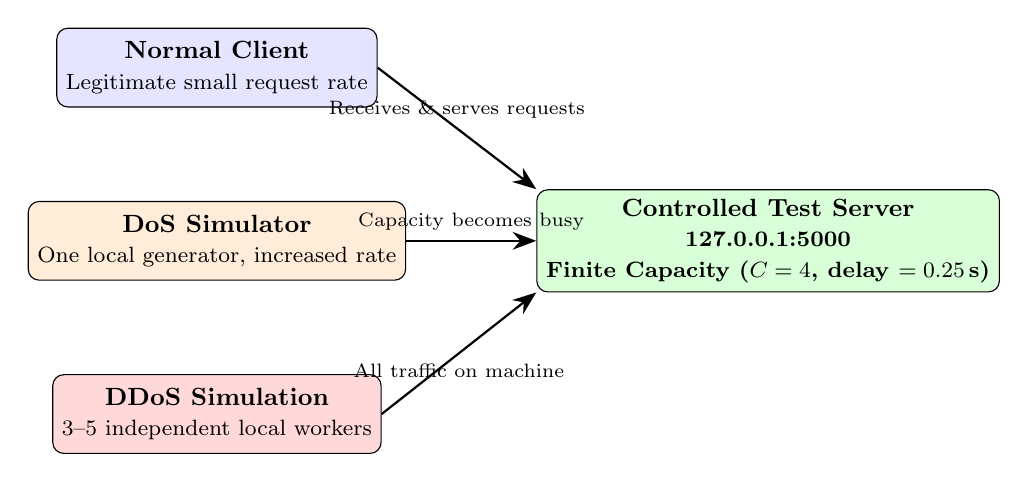
\begin{tikzpicture}[
    box/.style={draw, rectangle, rounded corners, fill=blue!10, minimum height=1cm, minimum width=3cm, align=center, font=\small},
    server/.style={draw, rectangle, rounded corners, fill=green!15, minimum height=1.2cm, minimum width=3.8cm, align=center, font=\small\bfseries},
    arrow/.style={-{Stealth[length=3mm]}, thick}
]

\node[box] (normal) at (0, 2.2) {\textbf{Normal Client}\\\footnotesize Legitimate small request rate};
\node[box, fill=orange!15] (dos) at (0, 0) {\textbf{DoS Simulator}\\\footnotesize One local generator, increased rate};
\node[box, fill=red!15] (ddos) at (0, -2.2) {\textbf{DDoS Simulation}\\\footnotesize 3--5 independent local workers};

\node[server] (target) at (7, 0) {\textbf{Controlled Test Server}\\\footnotesize 127.0.0.1:5000\\\footnotesize Finite Capacity ($C=4$, delay $=0.25\,\text{s}$)};

\draw[arrow] (normal.east) -- node[above, font=\scriptsize] {Receives \& serves requests} (target.north west);
\draw[arrow] (dos.east) -- node[above, font=\scriptsize] {Capacity becomes busy} (target.west);
\draw[arrow] (ddos.east) -- node[below, font=\scriptsize] {All traffic on machine} (target.south west);

\end{tikzpicture}
\caption{Conceptual topology for the controlled application-layer simulation.}
\end{figure}

\section{Experimental Setup}
\begin{itemize}[leftmargin=*]
    \item \textbf{Environment:} PC Localhost (\texttt{127.0.0.1}).
    \item \textbf{Software:} Python 3, Flask, Requests.
    \item \textbf{Server Capacity:} Deliberately set to $C = 4$ concurrency slots using \texttt{threading.BoundedSemaphore(4)}.
    \item \textbf{Processing Delay:} Artificial workload delay of $0.25\,\text{s}$ per request on the \texttt{/work} endpoint.
    \item \textbf{Safety Boundary:} Bounded request limits ($20$ to $100$ requests) strictly confined to loopback interface \texttt{127.0.0.1}.
\end{itemize}

\section{Implementation}
The experiment is organized into four core scripts:
\begin{enumerate}[leftmargin=*]
    \item \textbf{\texttt{server.py}:} Deliberately capacity-limited dummy Flask server recording accepted and rejected request counts. Exposes \texttt{/}, \texttt{/work}, and \texttt{/stats}.
    \item \textbf{\texttt{baseline.py}:} Sends 20 sequential requests with 0.15s delay to establish normal latency and 100\% success baseline.
    \item \textbf{\texttt{client.py}:} Single-generator DoS simulation dispatching 80 rapid requests with minimal delay (0.01s).
    \item \textbf{\texttt{ddos\_sim.py}:} Multi-source DDoS-style simulation spawning 4 independent worker processes sending 25 requests each (100 total concurrent requests).
\end{enumerate}

\section{Results \& Measurements}
The experiment was executed across the four defined stages:

\begin{table}[H]
\centering
\small
\caption{Experimental Measurement Results Across Stages}
\begin{tabular}{lcccc}
\toprule
\textbf{Metric} & \textbf{Stage A: Baseline} & \textbf{Stage B: DoS} & \textbf{Stage C: DDoS Simulation} & \textbf{Stage D: Recovery} \\
\midrule
\textbf{Total Requests}    & 20          & 80          & 100         & 15          \\
\textbf{HTTP 200 (OK)}     & 20 (100\%)  & 22 (27.5\%) & 25 (25.0\%) & 15 (100\%)  \\
\textbf{HTTP 503 (Busy)}   & 0 (0.0\%)   & 58 (72.5\%) & 75 (75.0\%) & 0 (0.0\%)   \\
\textbf{Errors / Timeouts} & 0           & 0           & 0           & 0           \\
\textbf{Average Latency}   & 264.4 ms    & 82.1 ms     & 93.0 ms     & 260.3 ms    \\
\textbf{Observation}       & Normal service & Capacity busy & Multi-source contention & Immediate recovery \\
\bottomrule
\end{tabular}
\end{table}

\noindent\textbf{Observation Analysis:}
\begin{itemize}[leftmargin=*]
    \item \textbf{Baseline:} All requests succeeded (100\% HTTP 200) with average latency reflecting the 250ms processing delay.
    \item \textbf{DoS Simulation:} Increased arrival rate from the generator exceeded available slots, causing 503 Busy responses for excess requests.
    \item \textbf{DDoS Simulation:} Four independent concurrent workers saturated the semaphore slots simultaneously, producing high 503 rejection rates.
    \item \textbf{Recovery:} Immediately after stopping the attack traffic, standard requests achieved 100\% success rate with normal latency.
\end{itemize}

\section{Comparison: DoS vs. DDoS}
\begin{itemize}[leftmargin=*]
    \item \textbf{DoS:} Single request-generation source. Demonstrates the basic principle of overloading a server from one origin.
    \item \textbf{DDoS:} Multiple independent worker processes simulating distributed sources. In this experiment, the DDoS part is simulated locally rather than performed against an external target.
\end{itemize}

\section{Defensive Measures}
\begin{itemize}[leftmargin=*]
    \item \textbf{Rate Limiting:} Restrict how many requests a client IP can make in a specified time window.
    \item \textbf{Connection/Worker Limits:} Prevent one source or burst from consuming every server worker thread.
    \item \textbf{Caching:} Serve repeated/static content without doing expensive backend computation each time.
    \item \textbf{Load Balancing:} Distribute legitimate traffic across multiple backend servers.
    \item \textbf{WAF / CDN / DDoS Protection:} Filter abnormal traffic upstream and absorb large traffic volumes.
    \item \textbf{Monitoring:} Watch request rate, latency, error rate, CPU, memory, and network usage.
\end{itemize}

\section{Ethical \& Safety Note}
The experiment was restricted to a self-owned localhost target (\texttt{127.0.0.1}) and bounded request counts. No public service or third-party system was targeted. No harmful lower-layer techniques (SYN flooding, UDP flooding, amplification, spoofing, botnet control) were used.

\section{Conclusion}
Increased concurrent request pressure caused requests to encounter the intentionally limited server capacity, demonstrating the availability problem that DoS and DDoS attacks exploit. When the attack ceased, the server recovered immediately, proving the importance of rate limiting and capacity management in production systems.

\newpage
\appendix
\section{Viva Preparation (Questions \& Answers)}

\begin{enumerate}[leftmargin=*]
    \item \textbf{What is the difference between DoS and DDoS?} \\
    \textit{Ans:} DoS comes from a single source; DDoS comes from multiple distributed sources, making IP-based mitigation harder.
    
    \item \textbf{Why does server capacity matter?} \\
    \textit{Ans:} Server resources (threads, memory, CPU) are finite. When arrival rate exceeds capacity, queues saturate and requests are rejected.
    
    \item \textbf{Why did we measure a baseline first?} \\
    \textit{Ans:} To establish normal performance under healthy conditions for accurate before/after comparison.
    
    \item \textbf{What does HTTP 503 mean in this experiment?} \\
    \textit{Ans:} It indicates the server's capacity semaphore was fully occupied, so the server rejected the excess request safely.
    
    \item \textbf{Why is our localhost DDoS only a simulation?} \\
    \textit{Ans:} Real DDoS attacks originate from distributed internet hosts; here, separate local processes simulate multiple sources safely on localhost.
    
    \item \textbf{What resources can a real DoS/DDoS exhaust?} \\
    \textit{Ans:} Network bandwidth, socket handles, CPU, memory, database connections, and worker threads.
    
    \item \textbf{How can a server defend against request floods?} \\
    \textit{Ans:} Using rate limiting, reverse proxies, caching, load balancing, autoscaling, and WAF/CDN scrubbers.
    
    \item \textbf{Why should an experiment be restricted to systems you own or have permission to test?} \\
    \textit{Ans:} Testing unauthorized systems is illegal, unethical, and disruptive. Localhost ensures total safety.
\end{enumerate}

\section{Source Code Listings}

\subsection{\texttt{server.py}}
\begin{lstlisting}[language=Python]
from flask import Flask, jsonify
import threading
import time

app = Flask(__name__)
CAPACITY = 4
PROCESSING_TIME = 0.25

slots = threading.BoundedSemaphore(CAPACITY)
stats = {"accepted": 0, "rejected": 0}
lock = threading.Lock()

@app.get("/work")
def work():
    acquired = slots.acquire(blocking=False)
    if not acquired:
        with lock:
            stats["rejected"] += 1
        return jsonify({"status": "busy", "message": "Server capacity is currently full"}), 503
    try:
        time.sleep(PROCESSING_TIME)
        with lock:
            stats["accepted"] += 1
        return jsonify({"status": "ok", "message": "Request processed"}), 200
    finally:
        slots.release()

@app.get("/stats")
def get_stats():
    with lock:
        return jsonify(stats)

if __name__ == "__main__":
    app.run(host="127.0.0.1", port=5000, threaded=True)
\end{lstlisting}

\subsection{\texttt{baseline.py}}
\begin{lstlisting}[language=Python]
import time
import requests

URL = "http://127.0.0.1:5000/work"
TOTAL = 20
latencies = []
success = failed = 0

for i in range(TOTAL):
    start = time.perf_counter()
    try:
        r = requests.get(URL, timeout=3)
        elapsed = (time.perf_counter() - start) * 1000
        latencies.append(elapsed)
        if r.status_code == 200: success += 1
        else: failed += 1
    except requests.RequestException:
        failed += 1
    time.sleep(0.15)
\end{lstlisting}

\end{document}
